\documentclass{article}

\title{Plausibly Realistic Sociotechnical Simulation with Aspect Orientation}
% Alternative titles:
%   Exploring the efficacy of aspect orientation in sociotechnical simulation
%   The use of runtime aspect weaving in simulation
\author{Tom Wallis}
\date{Forthcoming 2021}
\degree{Doctor of Philosophy}

% I heard you like ~~~CITATIONS~~~
\usepackage[
  backend=biber,
  bibencoding=utf8,
  style=ieee %% draft probably wants changing...
]{biblatex}
\addbibresource{refs.bib}


% Packages I for sure need
\usepackage{float}
\usepackage{graphicx}
\usepackage{titletoc}
\usepackage{enumitem}
\usepackage{csquotes}
\usepackage{xstring}

% Fonts
\usepackage[no-math]{fontspec}
\setmainfont{Valkyrie A}
\setsansfont{Concourse 4}
\setmonofont{Triplicate A Code}
\newfontfamily{\advocate}{Advocate55WideMed}
\newfontfamily{\concourse}{Concourse 4}
\newfontfamily{\concourseindex}{Concourse Index}

\usepackage{sectsty}
\allsectionsfont{\concourse}

% Listings config
\lstset{language=Python,
frame=L,
numbers=left,
stepnumber=1,
numberstyle=\footnotesize,
float,
floatplacement=H,
basicstyle=\normalsize\ttfamily}

% Extra colours for listings
\definecolor{backcolour}{gray}{0.95}

% Inline listings text size correction from https://tex.stackexchange.com/a/575053
\makeatletter
\lst@AddToHook{TextStyle}{\let\lst@basicstyle\ttfamily}
\makeatother



% For inline todos...nicked from https://tex.stackexchange.com/a/219354
\makeatletter
\usepackage{regexpatch}
\xpatchcmd{\@todo}{\setkeys{todonotes}{#1}}{\setkeys{todonotes}{inline,#1}}{}{}
\makeatother

% List formatting changes
\setitemize[1]{label={\concourseindex\normalsize\symbol{"2022}}}
\setitemize[2]{label={\concourseindex\small\symbol{"2022}}}
\setitemize[3]{label={\concourseindex\footnotesize\symbol{"2022}}}
\setitemize[4]{label={\concourseindex\scriptsize\symbol{"2022}}}
\setitemize[5]{label={\concourseindex\scriptsize\symbol{"2022}}} % Technically could be \tiny
\setenumerate[1]{font={\concourseindex\normalsize},label=\arabic*}
\setenumerate[2]{font={\concourseindex\small},label=\arabic*}
\setenumerate[3]{font={\concourseindex\footnotesize},label=\arabic*}
\setenumerate[4]{font={\concourseindex\scriptsize},label=\arabic*}
\setenumerate[5]{font={\concourseindex\scriptsize},label=\arabic*} % Technically could be \tiny

% Some quote styling changes, modified from https://tex.stackexchange.com/a/468294
\usepackage[%
linewidth=1pt,
middlelinecolor= black,
middlelinewidth=0.4pt,
roundcorner=10pt,
topline = false,
rightline = false,
bottomline = false,
rightmargin=0pt,
skipabove=0pt,
skipbelow=0pt,
leftmargin=-1cm,
innerleftmargin=1cm,
innerrightmargin=0pt,
innertopmargin=0pt,
innerbottommargin=0pt,
]{mdframed}
\makeatletter
%Take the original environment definition and change the leftmargin to 1cm
\renewenvironment*{displayquote}
  {\begingroup\setlength{\leftmargini}{1cm}\csq@getcargs{\csq@bdquote{}{}}}
  {\csq@edquote\endgroup}
\makeatother
%Hooks
%Use single spacing, set 10pt font, set quote style curly quotes, and beginning quotes
\renewcommand{\mkbegdispquote}
    {\begin{mdframed}\fontsize{12pt}{12pt}\setstretch{1.25}\setquotestyle{quote}\textooquote}
%End displayquote environment with ending quotes
\renewcommand{\mkenddispquote}{\textcoquote\end{mdframed}}


% Macros
% A todo system that is turned off by enabling final mode.
\makeatletter
\@ifclasswith{good_template}{final}
{\newcommand{\inline}[1]{}}
{\newcommand{\inline}[1]{{\color{red}{#1}}\addcontentsline{tdo}{todo}{#1}{}}}
\makeatother

\newcommand{\labelledsec}[2]{\section{#1}\label{sec:#2}}
\newcommand{\labelledsubsec}[2]{\subsection{#1}\label{subsec:#2}}
% a macro for indicating a number in an enumerated list using the concourseindex
% font (for consistency)
\newcommand{\pointno}[1]{{\concourseindex{}#1}}
% a macro to stop me switching between hyphenation/spacing/neither
\newcommand{\sociotechnical}{socio-technical }
% To prevent me absent-mindedly shortening pydysofu to pdsf, the macro is handy.
\newcommand{\pdsf}{PyDySoFu }


\newenvironment{researchquestion}{
  \begin{displayquote}\itshape
}{
  \end{displayquote}
}

\begin{document}

\maketitle


% ==============================================================================
\section{Introduction}
\label{sec:introduction}
Systems modelling is a fascinating field, largely as a result of its highly
interdisciplinary nature. This nature is both a blessing and a curse.\par

On one hand, the breadth of the field gives a range of diverse problems to work
on, and many interesting research opportunities spring forth as a result. At the
same time, this scope breeds a host of different philosophies regarding systems
modelling, often muddying the waters with regards the field's literature. This
can make identifying small-scale, incremental improvements on the existing
literature hard to identify. Fortunately, the Cambrian explosion that is modern
systems research provides an opportunity to do research which can make tangible,
genuine improvements to everyday life.\par

This work began by investigating different ways to model systems, with an eye to
compose together or translate between different modelling paradigms. As reading
the literature exposed potential research opportunities which were eliminated
after some investigation, the work took on an exploratory nature before recently
resting at a well-scoped and viable research opportunity. This report will
discuss that work chronologically, reviewing the initial literature in
\cref{part:model_transformations}, discussing the later exploratory work in
\cref{part:exploratory_development}, and finally ending with a discussion of the
final research topic in \cref{part:resilience}.


\part{Model Transformations}
\label{part:model_transformations}
% ==============================================================================
\section{Systems Modelling Literature}
\label{sec:literature}
The diversity of system modelling requirements results in a variety of
philosophies regarding what models should look like. A useful distinction
between these philosophies is their take on the traditional input, process,
output concept; different modelling paradigms capture information in
different ways, allow varying degrees of analysis to be performed on this
captured information, and lend themselves to different methods for the
exposition of the results of this analysis.\par

Given different approaches exist for these fundamental aspects of models, a
question arose: is it possible to make use of the strengths of different
paradigms by translating between them? The following review of relevant
literature explores this possibility.\par


\subsection{UML, SysML \& OPM}
\label{subsec:uml}
One approach to modelling systems is the diagrammatic one taken by
UML\cite{rumbaugh2017unified}, which is the de-facto modelling framework for
software architectures. UML has been refined gradually over around 25 years, and
has grown to model a variety of systems.

UML's origins are in mapping the structure of software, but it can now be used
to model a variety of more general systems via SysML\cite{sysml_spec}. A
comparison between this and its early competitor, OPM\cite{dori1995object},
which also models a variety of systems, can be enlightening.\par

Where UML's expressiveness comes from an array of diagram types and extensions
to its ordinary diagrams --- such as SysML --- OPM uses a more curated set of
building blocks to build models from, gaining expressiveness with a simpler
modelling system. These building blocks are structured objects of information,
and processes that the information is transformed by --- concepts which prove to
be rather universal, as seen in OPM's cross-disciplinary
appeal\cite{opm_bio_research}. OPM's native focus on processes and simple
fundamental units delivers the useful feature that OPM models are generally
\emph{executable} for analysis, allowing deeper insights into the subject of
the model.\par

This simplicity is often cited as a benefit of OPM: there is less for a modeller
to learn, and the core concepts building the framework are powerful. However,
while both are recognised standards (UML is a standard supported by the Object
Management Group, where OPM is supported by ISO), UML seems to see much wider
industrial use. We might suggest that this is actually \emph{because} of the
additional diagram classes in UML: each diagram class becomes slightly simpler
than an OPM diagram, and the result is that each diagram comes with its own
visual identity. This imparts lots of context about what the model is displaying
to a viewer at a glance, and reduces the amount of friction involved in the
modelling process.\par

The amount of context available at a glance turns out to be especially important
for UML, because UML can rarely be formally processed for analysis. Instead,
results of the UML modelling process are typically done by a visual analysis of
a diagram.\par

UML is capable of dealing with a variety of socio-technical, hard-to-define
systems via its different diagram types and can work at a variety of resolutions
of detail, making it adept at handling ``black boxes''. However, as scale
increases, so does the number of diagrams --- a problem shared by OPM --- which
can make it intractable to use at scale.\par

% ===== OBASHI
\subsection{OBASHI}
\label{subsec:obashi}
A modelling platform which attempts to fix this problem of diagramming at
scale is OBASHI\cite{obashi_methodology}. OBASHI sees industrial use for the
specific task of modelling dataflow in socio-technical systems. Like UML,
OBASHI's modelling paradigm is entirely graphical. Models have simple
fundamental components --- ``elements'' and six kinds of ``relationships'' ---
which are composed together according to a series of rules. Elements are
separated into ``layers'', and an ordering is imposed which groups social and
technical kinds of elements separately, mediating dataflow between them via
business processes.\par

The modelling system is proprietary, and a tool is available from the company
developing the methodology. This tool can perform some automated analysis on an
otherwise graphical system model, such as impact analysis of element failure or
the generation of different diagrams representing different potential pathways
for dataflow between elements.\par

OBASHI takes an interesting perspective on the difficulties of modelling
hard-to-define systems, as the design of its diagrams is specifically
constructed to cater to non-technical recipients of diagrams. As the outputs of
analysis are often more diagrams, the diagrams that are produced are laid out in
such a way that stakeholders in a diagram who are unfamiliar with the nuances of
their subject can still understand the implications of an analysis. This is
possible, however, because OBASHI is capable of modelling only systems which
permit the flow of information or data --- this limitation in scope allows
OBASHI to successfully address many of the difficulties of informal modelling at
scale, at the cost of flexibility.\par

% ===== BPMN
\subsection{BPMN \& BPEL}
\label{subsec:bpmn}
A popular alternative to both UML and OBASHI for business process modelling is
found in BPMN\cite{bpmn_intro}. BPMN is generally a graphical modelling
framework, with a language to support executable process definitions via its
companion language, BPEL\cite{bpel_1.1_spec}. Not unlike OBASHI, BPMN aims to
demonstrate concepts graphically in a simple enough format that non-technical
recipients of diagrams can understand their meaning. BPMN can be considered the
business equivalent of UML, and is also supported by the Object Management
Group.\par


% ===== Bigraphs
\subsection{Bigraphs}
\label{subsubsec:bigraphs}
A convenient segue from these informal modelling techniques to formal ones are
bigraphs, in that, to a degree, Bigraphs support both formal \emph{and} informal
paradigms. This is because bigraphs are defined in three ways:

\begin{enumerate}
\item As a graphical notation, easily visually parsed
\item As an equivalent algebra
\item As a category in category theory
\end{enumerate}

As a result of a carefully constructed mathematical definition, bigraphs have
the capacity to cope with often complicated features, such as safely composing
systems together, or the formal manipulation of a system's structure. This
formal foundation can make bigraphs complex to use for a non-technical
modeller. Fortunately, the graphical notation for bigraphs is both simple and
expressive.\par

Bigraphs are often discussed as having both \emph{space} and
\emph{motion}\cite{milner2009space}. The \emph{space} of a system is defined by
Robin Milner (the original designer of the bigraph formalism) as the placements
of nodes relative to each other. This is represented, mathematically, as a
forest of nodes. Parental relationships in a given tree in the forest represent
containment of one node inside another.\par

The \emph{motion} of a model is defined as how the model changes over time.
Milner represents system behaviour as change according to \emph{reaction rules}:
patterns which match on a subgraph of a ``complete'' bigraph, and dictate how
the matching subgraph looks in a future iteration of the bigraph. Reaction rules
turn out to be rather powerful, and can represent any system within a category
of systems called a \emph{bigraphical reactive
  system}\cite{milner_early_brs_definition} (BRSes). BRSes can represent a
number of calculi, including \picalculus{} and the ambient
calculus\cite{bigraphs_and_transitions_milner_jensen}.\par



% ===== Petri Nets
\subsection{Petri Nets}
\label{subsubsec:petrinets}
As an alternative to bigraphs, system modelling can be done formally via methods
such as Petri Nets\cite{petri_net_seminal}. A Petri Net is a directed graph of
states and processes those states can undergo to reach future states. Petri Nets
were born initially out of chemistry literature\cite{petri_net_seminal}, but
have seen applications in areas as diverse as workflow
modelling\cite{petri_net_workflow_modelling},
concurrency\cite{petri_net_concurrency}, and molecular networks in systems
biology\cite{petri_nets_for_biology}.\par

Petri nets have similarities with OPM, as they are both fundamentally concerned
with state (arbitrary state in the case of Petri Nets, and a more specific state
of structured data in the case of OPM) and processes that their states go
through. An interesting topic of research could be the combination of the two,
given their commonalities, which could eventually lead to a relatively
high-level modelling system with a powerful mathematical framework underlying
it.\par


% ===== CAS modelling via pdes, cellular automata...
\subsection{Complex Adaptive Systems Modelling}
Complex Adaptive Systems (CASes) are a category of systems with typical traits
of parallelism, conditional action, modularity and adaptation or evolution\cite{holland_studying_adaptive_systems}.
While CASes are prevalent in everyday life and the subject of much study, their
modelling is difficult and elusive due to a few factors, and many open problems
persist in modelling efforts for these systems\cite{gell-mann}.\par

CASes hold lots of important relevant detail which greatly affects the dynamics
of a model; as a result, they cannot be adequately modelled by most informal
modelling paradigms. They also difficult to process or model in a mathematical
way, however, as producing a coherent and verifiable mathematical model of these
systems is generally intractable or impossible due to their non-linear
behaviour\cite{holland_studying_adaptive_systems}.\par

Mathematical models can therefore be made in certain cases, but alternatives are
necessary. A typical method for modelling --- and investigating the behaviour of
--- CASes is to use agent-based modelling\cite{hewitt}. This can be done in
several ways, the most common being to write a bespoke model in code, often in
an agent-based framework such as Theatre~\cite{theatre_repo}, or by writing in
an automata or agent-oriented modelling language, such as
NetLogo\cite{netlogo}.\par


\subsection{\pdsf{}}
\pdsf{} is library developed in earlier, related research projects, designed for
modelling variance in behaviour as a cross-cutting concern in Python via
aspect orientation~\cite{aspect_orientation}. \pdsf{} uses ``fuzzers'' ---
transformations on an Abstract Syntax Tree (AST) --- to alter Python methods
before they are run. Method invocation is interrupted, and the Python code
associated with the method replaced with a ``variant'' --- the result of passing
the original AST of the method through its associated fuzzer. This allows it to
manipulate models repeatedly during model execution, referred to as ``dynamic
fuzzing''.\par

Modelling using \pdsf{} doesn't require a certain modelling paradigm to be
followed, meaning that any paradigm implementable in Python can be integrated
with the tool. However, it lends itself particularly well to agent-based
modelling, and can be used easily in tandem with Theatre. This has already been
used in an exploration of software development workflows\cite{caise_forum_18}.
\pdsf{} is explored in depth in \cref{part:two}.\par

\subsection{Findings after Evaluating the Literature}
A significant amount of time was spent evaluating the available literature,
trying to investigate research opportunities in the construction of system
models. The idea of translating system models from one model type to another was
of particular interest, so as to simplify the capture of system detail in some
areas and to simplify analysis in others.\par

Several approaches were investigated. One was the translation between OBASHI and
bigraphs: bigraphs offer powerful encoding of behaviour via reaction rules, and
have many formal components, features OBASHI trades for high-level modelling and
elegant visualisation, which is an improvement area for bigraphs. Translation
could pair the capture \& display advantages of OBASHI with the analytical
capacity of bigraphs' formal foundations. It became clear after some initial
prototyping, however, that OBASHI represents lots of information which is
possible but inefficient to encode in a bigraph. Similarly, bigraphs represent
information which cannot be stored in an OBASHI diagram. While some modelling
platforms are supersets of others, bigraphs appear insufficient as an
intermediate form for the modelling of high-level frameworks.\par

As model transformation concepts were explored more, another issue became
apparent, which was that encoding information in one paradigm might have
different \emph{contextual} meaning than others. That is, the same model
component --- such as a node on a graph --- might ``mean'' different things to
different system architects. To draw further examples from the comparison of
OBASHI and bigraphs, OBASHI represents lots of important data surrounding model
structure as attributes on the vertices and edges of their graphs; bigraphs
permit no information on edges, but after discussions with bigraph researchers,
it became apparent that this would typically be represented as further
information on additional nodes on edges (made even messier by bigraphs' lack of
a type system). Semantic differences between architects who use different
paradigms would cause incompatible mental models of what a model represented.
The same model \emph{must} be interfaced with in both paradigms, because
necessary details for some target paradigm would be impossible to represent via
some paradigms used to capture initial information.\par

Another approach investigated was for \pdsf{}, together with Theatre, to act as
a universal target for other modelling paradigms to translate to --- this was
also unsuccessful. While many (if not most) modelling paradigms seem to be
representable as a combination of an actor model and dynamic fuzzing,
uncertainties about what different model components \emph{meant} caused this
idea to be discarded. The reasoning was that using \pdsf{} as a universal
intermediary was really useful when it permitted different parts of a model,
represented in two different paradigms, to be combined by translating to
\pdsf{}. However, concepts between the two original paradigms can contain subtle
differences, leading to inconsistencies which are hard if not impossible to
eliminate without strict formal definitions of all original representations. As
many representations of systems are \emph{informal}, this research idea was also
eliminated.\par

After much exploration and little resulting direction, a new angle was
attempted. \pdsf{} is capable of dynamic fuzzing, a property not seen in any other
modelling paradigm reviewed\footnote{Technically, bigraphs get close, as the
  BigraphER\cite{BigraphER} modelling framework has an undocumented API for
  turning on and off reaction rules. Whether this would suffice for dynamic
  fuzzing implementations is unclear, but this certainly is not part of the
  original bigraph spec.}. To discover interesting research possibilities
concerning \pdsf{}, some exploratory development of the tool was performed.\par


\part{Exploratory Development}
\label{part:two}
\label{part:exploratory_development}
% ==============================================================================
\section{\pdsf{}'s initial state}
\label{sec:pydysofu}
\pdsf{}'s original version was a small Python decorator for socio-technical
modelling, called \emph{fuzzi moss}\cite{honours_thesis}. Since this initial
development, \pdsf{} had gone through a series of improvements before this
project began, culminating in a separation of the core dynamic fuzzing
capacities from the socio-technical components of the tool. Rather than a tool
for dynamic fuzzing, Fuzzi Moss had become a suite of fuzzers for
socio-technical simulations built on top of \pdsf{}, which implemented dynamic
fuzzing.\par

Some types of socio-technical behaviour, however, were difficult if not
impossible to implement via \pdsf{}'s method for fuzzing. Specifically,
habit formation and complex conditional fuzzing were difficult if
not impossible to implement via \pdsf{}'s approach, because:

\begin{itemize}
\item It wasn't possible to specify, via one of \pdsf{}'s aspects, future
  fuzzing based on the previous return value of a target.\\
  This is important, because we often alter a workflow in real-life systems when
  we know what the outcome of a previous change is. For example, after a
  workflow change leads to an unsafe situation in a safety critical system such
  as a rail network, the agent concerned is likely to amend their behaviour in
  future.
\item It wasn't possible to develop fuzzers which had a native concept of state
  over time. That is: fuzzers could be considered as graph transforms, which
  were completely unaware of previous variants developed. Implementing this
  would make solving the issue above easier also. This was important, because
  there are scenarios where adaptation in a socio-technical system is unlikely
  to occur for a second time if it's already been tried, or if the adaptation
  led to poor results in the past.
\end{itemize}

Both issues were resolved by separating \pdsf{}'s fuzzing capabilities into a
package of its own, and solving these problems on the level of aspect
  orientation. Rather than iterating on \pdsf{}, \pdsf{} was built as
a collection of ``fuzzing aspects'' implemented in a framework which
splintered from \pdsf{}'s codebase, called ``ASP''.\par


\section{ASP}
ASP\cite{asp_repo} is an aspect orientation framework written in python,
exploiting the technique which permitted \pdsf{} to operate in the first
place.\par

Where \pdsf{} injected functionality into an overridden
\texttt{\_\_getattribute\_\_} definition, ASP does the same --- but where
functionality was represented as a \emph{function} which transformed an AST, ASP
fuzzes using \emph{objects}. If these objects have special methods defined, ASP
injects functionality according to those methods. The special methods it picks
up --- \texttt{prelude}, \texttt{encore}, \texttt{around}, and
\texttt{error\_handling}, are detailed in appendix 1.

In implementing these pieces of functionality, the foundation for \pdsf{} became
an aspect orientation library capable of capturing return values of fuzzed
functions, and storing information pertinent to the fuzzing process --- in
particular, results and the variants that produced them --- in the fuzzer's
internal state, because fuzzers can now be objects satisfying the requirements
for ASP to use them as aspects.\par

The work remaining at this stage was to rewrite \pdsf{}'s fuzzing procedure to
be built on top of ASP.\par


% ==============================================================================
\section{Improvements to \pdsf{}}
\label{sec:pdsf_improvements}
As the above work satisfied the requirements for more complex fuzzing to be
built using \pdsf{}, the stage had been set to rewrite the library's core
functionality on top of ASP. Implementation of the previous functionality in
\pdsf{} turned out to be the implementation of a single class, which could reuse
existing \pdsf{} mechanisms, an example of which can be found in appendix 2.\par

A benefit of ASP's object-oriented approach is that additional functionality can
be implemented by simple subclassing of the original \texttt{FuzzingAspect},
where a call to the \texttt{self.apply\_fuzzing} method can apply actual fuzzing
functionality, leaving the subclass concerned only with additional features.\par

New fuzzers, implementing more complex behaviours, were then implemented and
tested. Specifically, the \texttt{IncrementalImprover} fuzzer class generates
\emph{multiple} variants of a target, and fuzzes in a manner similar to the
above\footnote{As the code for \texttt{IncrementalImprover} is long and complex,
  it has been omitted here, but can be found in the project
  repository\cite{pydysofu_repo}.}. However, \texttt{IncrementalImprover} makes use
of ASP's introduction of catching return values to record the success of
different variants, and to generate future variants by applying fuzzing to
successful previous variants.\par

This additional functionality is especially important for more complex
socio-technical simulations. For example: \pdsf{}'s original functionality
permitted the same function to be fuzzed again and again with random results
each time, but fuzzing could not be stacked across multiple invocations of a
workflow step, i.e. introducing variance once, and then introducing further
variance where previous variance \emph{persisted}.\par

The \texttt{IncrementalImprover} is therefore a proof-of-concept for more
sophisticated simulations of socio-technical variance and --- while the
functionality has not yet been introduced into Fuzzi Moss --- it is intended to
permit simulations specifically around instances of variance such as habit
formation.\par


\section{Segue: Genetic Programming}
% ReaLX submission stuff
The implementation of incremental improvement rested on the ability to track
previous variants, and to record which variants were more ``successful'' than
others. It is clear to see that there is a similarity between the requirements
of the \texttt{IncrementalImprover} and that of genetic programming, then, as
genetic programming approaches to solving problems must construct many different
representations of processes and compare them for ``fitness''.\par

Genetic Programming approaches are often used to improve the state of an
existing codebase\cite{locoGP}\footnote{No term for this
  specific field was found. It will be referred to here as ``genetic
  metaprogramming''.}. Interestingly, genetic metaprogramming has been performed
similarly to how \pdsf{} operates already, by the modification of an
AST\cite{locoGP}, but --- like much of genetic metaprogramming literature ---
the technique is used to improve a codebase. An alternative approach presents
itself as a variant of what the \texttt{IncrementalImprover} was originally
intended to do: generate many variants of a single function, check its
``fitness'' against some success metric, and continue to fuzz successful
variants in future generations. This approach takes the typical AST-style
genetic modification, and employs it to attempt to solve regular genetic
programming problems.\par

Symbolic regression, a canonical genetic programming problem, was attempted
using this alternative technique to traditional genetic programming angles (such
as constructing a tree representing a solution to a
problem\cite{koza1994genetic}, or constructing more sophisticated directed
graphs\cite{cartesian_gp}). These
techniques inherently attempt to solve problems in a somewhat functional style.
Dynamic fuzzing, however, allows an imperative-style solution to a problem to be
engineered, where things like state can be manipulated by the solution via the
AST. Some variants of genetic programming, such as stack-based genetic
programming, also attempt this\cite{stack_based_gp} but ultimately rely on the
same fundamental functional style of other approaches.\par

Implementing genetic programming in \pdsf{} did not require a significant amount
of change to the library once the \texttt{IncrementalImprover} had been
implemented. Changes in ASP and \pdsf{} to permit fuzzers which could record a
history of their fuzzing were sufficient to implement a
\texttt{GeneticImprover}, by subclassing the \texttt{IncrementalImprover}. As
new rounds are generated in the \texttt{GeneticImprover}, successful previous
variants are not just kept, but their ASTs spliced together to mimic the
recombination performed when comparing tree solutions in ordinary genetic
programming\cite{koza1994genetic}. A symbolic regression converging to typical
test polynomials was implemented using this to confirm that it worked as
intended, the source of which can be found in the \pdsf{}
repository\cite{pydysofu_repo}, and a paper outlining the work in more detail
found at \cite{realx_paper}.



\part{Resilience}
\label{part:resilience}
\section{Direction Change}
Evidently, \pdsf{}'s core concept --- dynamic fuzzing --- is applicable to many
different fields, and poses a variety of research opportunities, including:

\begin{itemize}
\item Use for introducing variance to socio-technical
  simulations\cite{honours_thesis}
\item Implementation of Genetic Programming\cite{realx_paper}
\item Design of aspect orientation frameworks capable of modifying their targets
  directly, rather than wrapping them, as is the case with traditional AOP
  techniques\cite{aspectj}.
\item Use for simulating changing behaviour in a complex adaptive system
\end{itemize}

A choice of direction therefore had to be made. As a library of socio-technical
fuzzers already exists\cite{fuzzi_moss_repo}, and some preliminary work had been
done in simulating software development methodologies exposed to socio-technical
stress, this seemed an appropriate path to continue along. This was influenced
in part by the fact that, in the interim period between the initial work on
\pdsf{}\cite{honours_thesis} and the beginning of this study, a more in-depth
simulation of development methodologies under socio-technical stress had been
developed. Earlier this year, a paper on the work was
published\cite{caise_forum_18}.\par

Feedback from the submission of that paper had outlined some core issues which
had to be addressed. For one, validating the work against verifiable industry
data was difficult: some process logs for industry exist in public, but they are
uncommon. It can therefore be difficult to verify the problem domain's validity
\emph{before} verification. This is discussed more in \cref{sec:research_risks}. In
addition, the fuzzers used in \cite{caise_forum_18} were called into question,
as they weren't validated as being representative of the behaviour being
simulated.\par

Further work building on these simulations did present itself, however.
Particularly, more sophisticated variance introduced to the models which made
use of the new technologies in \pdsf{} --- particularly the potential to model
habit formation --- present themselves as future work building on the
already-published material. To perform this research properly would require a
degree of rigour and detail which was not present in the initial study of
variance as a cross-cutting concern.\par

Further work on the topic could be, then, to develop sophisticated models of
socio-technical systems for use in later experimentation. These could be
verified by experts in the domain. The same could be done for more advanced
fuzzers, working with researchers in Psychology to ensure that the variance
represented by the fuzzer was indicative of the variance seen in the real world.
The result would be an accurate and validated model of socio-technical variance,
which could prove otherwise elusive.\par

This foundation then paves the way for more complex experimentation. Emergent
phenomena could be spotted in socio-technical systems under stress that might
not be spotted without accurate simulation of that stress. For example:
safety-critical system literature makes reference to the states that systems
enter when agents make simplifications to a procedure which, while innocuous on
their own, interact to cause parts of a system to fail, often leading to unsafe
systems\cite{johnson_shea_rail}. Degraded modes are a mechanism which can
preserve vital system components until --- ideally --- failing components are
put right. Once a verified model of a system under variance is developed, then,
sophisticated assessments of the system's \emph{resilience} under
socio-technical stress can be simulated.\par

This technique could prove useful in a pragmatic sense, in industry: systems put
in place in healthcare, public infrastructure, business systems such as supply
chains, communication networks, and a host of similar real-world systems exhibit
variance, but actively testing systems under different kinds of variance can be
elusive as variance is difficult to model without treating it as a cross-cutting
concern\cite{caise_forum_18}. Performing a monte-carlo simulation on a
simulation under different kinds of stress, or the same stress under different
initial conditions, or the same stress \emph{and} initial conditions with
differing random seeds to represent real-world unpredictability, could allow a
proposed system to be probed for flaws by assessing how well it holds up in
real-world scenarios. Where socio-technical variance can be modelled as a
cross-cutting concern separated from any given domain model, a library of
variances can be composed, and then applied to a problem domain to probe its
resilience under socio-technical stress by plugging a problem domain into a
suite of tests. the research is instead motivated by a seeming lack of these analyses in
existing literature, and an opportunity to marry this research with industry
requirements.\par



% ==============================================================================
\section{Notes on Resilience}
\label{sec:resilience}
Resilience is a complicated subject, affecting myriad fields. For example,
system science is sometimes concerned with resilience regarding robustness of
socio-technical systems for the purpose of security
analysis\cite{bloomfeld_boundaryless_resilience}.

A more theoretical angle is taken in the domain of resilience
engineering\cite{hollnagel_leveson_woods} investigates how to construct systems
which are resilient by design. Resilience within systems can be evaluated
according to various properties, such as --- as per the Resilience Analysis
Grid\cite{hollnagel_RAG} --- its ability to ``respond, monitor, learn, and
anticipate''\footnote{It is difficult not to see some parallels between these
  four traits and the improvements to \pdsf{} made possible by ASP.}. Indeed,
finding literature on quantitative methods for resilience engineering proves
fruitless, though qualitative perspectives are plentiful. This research direction
was chosen fairly recently, however, and so more reading is required for a
firmer grip on the current state of resilience in system science.\par

Other fields take alternative approaches in assessing resilience. Of particular
interest is the angle taken by design. For some in the field, ``smartness
produces resilience''\cite{halpern_grey_room}, concerning the aims of IBM for
the last decade; other design approaches aim to work in the service of more
resilient ecosystems\cite{public_sediment}.\par

What makes design so interesting as a repository of literature on system
resilience is the field's increasingly deep connection to industry and practical
work\footnote{Though practical and pragmatic aren't necessarily the same
  thing.}; design is increasingly focused around the implementation of solutions
to problems identified in the world via the application of ``systems thinking''.
Where many scientific articles on resilience, and system science generally, are
retrospective analyses of relevant scenarios(such as \cite{johnson_shea_rail})
or theoretical in nature(such as \cite{statistical_physics_self_replication}),
design work often \emph{proposes implementable solutions}, using the theory from
relevant fields such as systems theory and cybernetics, to fix problems raised
by these retrospective analyses.\par

In many ways, design has evolved to become the hands by which system science and
its related fields mould the world.\par

This research project is squarely rooted in computing science, however, and a
focus on design will serve to distract more than to inform. Still: an awareness
of the field helps to guide this research in helpful directions. Integrations
with existing design methods, and an understanding of how modelling is often
performed --- qualitatively \emph{and} quantitatively --- can help develop
research with industrial relevance that can support future work.\par

Importantly, different fields take different approaches to what resilience
\emph{means}. Within computing science, for
example\cite{biology_software_same_coin}:

\begin{displayquote}
  \ldots{}the ability of a system to persistently deliver its services in a
  dependable way even when facing changes, unforeseen failures and intrusions.
\end{displayquote}

However, for the socio-technical systems we intend to model here, Hollangel's
definition feels more appropriate\cite{hollnagel_RAG}:

\begin{displayquote}
   A system is said to perform in a manner that is resilient when it sustains
   required operations under both expected and unexpected conditions by
   adjusting its functioning prior to, during, or following events (changes,
   disturbances, and opportunities).
\end{displayquote}

Being aware of what we mean when we talk about resilience is clearly essential
for this research. Some immediate next steps for this project as it orients
itself around resilience are:

\begin{enumerate}
\item Process additional literature surrounding resilience
\item Especially, investigate quantitative measures of resilience
\item Identify the theoretical and tooling-based contributions the research can
  make, keeping it within domain, while increasing how evaluable it is by
  considering how design makes system science pragmatic
\end{enumerate}


% ==============================================================================
\section{Future Plan}
\label{sec:future_plan}

% Validated model of behaviours (Lego)
The first step of expected future work is to construct a validated model of Rob
Dekkers' game for teaching applied systems theory to undergraduate students.
As Rob Dekkers teaches within Glasgow University, and is the second supervisor
for the project, validation of the problem domain should be achievable. The game
is small-scale enough to be run as experiments which can produce empirical data
to test against. The game's resilience to variance on the part of the students
can be assessed.\par

% Validated Model of behaviours (Information systems, using available process
% logs)
This can be done alongside the development of models based on available process
logs. Some information system logs \emph{are} available, providing more
empirical data to validate against. This can provide a second case study,
providing additional problem domains which verified variances can be later run
against. Effectively, this can be considered a more rigorous version of the
study undertaken in our earlier work\cite{caise_forum_18}.\par


% Validated variances, including more complex variances
As \pdsf{} now has the capacity to simulate more complicated variances, these
variances will need to be validated by experts in psychological domains in much
the same way that socio-technical system models need to be validated by experts
in their domains. Fuzzers representing more sophisticated real-world variance,
such as habit formation, must be developed for the investigation of large-scale
system modelling with variance, and these must be validated by working alongside
psychologists (or experts in similar fields) who can assess that fuzzers
represent the variance they are intended to.\par


% Model of habit-forming variance (NHS? Safety-critical Systems?)
Once more complex fuzzers have been developed, and moderate-scale models
developed and used as a testing ground for assessing resilience, industry-scale
models can be developed, verified with industry, and pre-verified fuzzers
applied to these real-world workflows to test their resilience. This large-scale
project will take longer and require rigour and industry collaboration;
potential to perform these experiments with system design currently underway in
the NHS has been identified, and efforts to make contacts in this project are
already underway so as to avoid later delay.\todo{Gotta get me one of those good
Gantt charts...}\par



% ==============================================================================
\section{Thesis Statement}
\label{sec:thsis_statement}
Resilience as an emergent property of a socio-technical system can be difficult
to reason about quantitatively, as gathering information around a system's
resilience to stress typically means either constructing complex models
including variance and uncertainty in the problem domain, or exposure of a
prototype system to real-world scenarios, both of which are impractical to build
and intractable to validate.\par

Dynamic fuzzing offers a solution. Introducing variance as a cross-cutting
concern reduces the complexity of resulting system models, permitting simpler
problem domains and implementations of variance. The simplicity of each
component permits tractable model validation in turn. Validated models can then
be experimented on, and the model's resilience to socio-technical stress
quantified. Where variance is modelled in non-domain-specific ways, suites of
tests can be built for socio-technical systems where verified domain models can
be exposed to a simulation of real-world variance, and their response to that
variance realistically measured or asserted.\par


% ==============================================================================
\section{Risks and Mitigating Actions}
\label{sec:research_risks}
One significant risk to the project is that many enticing directions are
available, as dynamic fuzzing appears to be a versatile and useful technique
with many exciting applications\footnote{Some potential future work deemed out
  of scope can be found in appendix 3.}. It will therefore be important to keep
in perspective the balance between breadth and depth required of a PhD. In an
effort to stay focused, the project has been planned out with its constituent
case studies, so as to maintain direction when other interesting research
opportunities present themselves. A Gantt chart of this project plan can be
found in appendix 4.\par

Another risk is that verifying and validating systems science with empirical
data is very difficult, and designing scientifically valid experiments around
system science is a challenge. To aid this, process logs and similar evidence
are intended to be used wherever available, and the project has been planned
around the availability of empirical data in an effort to produce scientifically
valid results. In an effort to assist experimental design, \pdsf{}'s original
aspect oriented design was capitalised on as it underwent changes during the
initial phases of this project. Hypotheses around resilience are to be written
as unit tests against the problem domain, where resilience is being tested in
the presence of certain variances; this variance is introduced as a
cross-cutting concern via ASP, making the body of the unit test an experiment
which can pass or fail. It is hoped that this makes the construction of
experiments clearer, and should simplify the domain model\cite{caise_forum_18},
making the model easier to validate with experts.\par



% ==============================================================================
\section{Conclusion}
\label{sec:concluion}

The project has undergone a radical shift in direction in a relatively late
stage. Ultimately, the back-and-forth of exploratory work yielded a paper
submission\cite{realx_paper}, a number of identified research directions, and
perspective on the systems modelling field and the angles that
might be both fruitful and suitable to PhD research.\par

With this perspective, a new research angle has been devised. The new angle
addresses opportunities both in literature and in industry, has a more
appropriate scope than previous directions, and acts as a continuation of
existing work in the project\cite{caise_forum_18}. The interruption of direction
has, however, limited available time and left the project with less practical
work than was hoped at this stage. The next step is therefore to engage with
case studies similar to those previously attempted, and with researchers within
the university.\par

All research comes with risk; this is no exception. The risk in this research is
not out-of-the-ordinary, though: many of the potential issues arise not out of
the direction of this research, but the general field that the research exists
within. Where this research does yield unique risks, measures are actively
planned to reduce the risk and ensure that the research moves smoothly. In
addition --- because no plan is perfect --- the project plan for this research
includes periods of margin time where unforeseen circumstances can consume
additional time without upsetting the overall timeline for the project.\par

Finally: \pdsf{} presents a series of remarkably exciting research directions,
and it is regrettable that only one can be chosen! It is hoped that alternative
uses for the library will be attempted by other researchers or as parts of
student projects.\par





\bibliography{lib}





% ==============================================================================
\appendix
% ==============================================================================

\newpage
\section*{Appendix 1: \pdsf{} Special Methods}
\label{app:special_methods}

\begin{description}

\item[prelude(attribute, context, *args, **kwargs)] \hfill \\
  A \texttt{prelude} method on an object passed in as a fuzzer will run
  \emph{before} the target function is run. It has access to the target
  attribute, and to the original object the target is tied to in a
  \texttt{context}. It can also inspect the arguments the target function will
  be given.

\item[encore(attribute, context, result)]\hfill \\
  An \texttt{encore} method on an object passed in as a fuzzer will run
  \emph{after} the target function is run. It has access to the target
  attribute, and to the original object the target is tied to in a
  \texttt{context}, as well as the result of the target..

\item[around(attribute, context, *args, **kwargs)]\hfill \\
  An \texttt{around} method on an object passed in as a fuzzer wraps the target
  attribute in functionality which comes before and after it is executed. This
  can be used as an alternative to \texttt{encore} and/or
  \texttt{prelude}.\\
  An \texttt{around} method gets the same signature as the \texttt{prelude},
  because it must have at least the same functionality as a \texttt{prelude}
  method, but does not require the result of execution passed in as \emph{around
    is expected to execute the target attribute, with the arguments provided.}\\
  Worth noting is that if \texttt{around} exists at the same time as one or more
  of \texttt{prelude} or \texttt{encore}, then \texttt{prelude} or
  \texttt{encore} will be wrapped around the \texttt{around} method.

\item[error\_handling(attribute, context, exception)]\hfill \\
  An \texttt{error\_handling} method on an object passed in as a fuzzer will
  catch exceptions raised by the target attribute and attempt to handle them
  elegantly. This is a common piece of functionality in other aspect orientation
  frameworks\cite{aspectj}.

\end{description}


\newpage
\section*{Appendix 2: \texttt{FuzzingAspect} Implementation}
\label{app:fuzzing_aspect}

\begin{figure}[H]
  \begin{lstlisting}

from asp import IdentityAspect
    
class FuzzingAspect(IdentityAspect):

    def __init__(self, fuzzing_advice):
        self.fuzzing_advice = fuzzing_advice

    def prelude(self, attribute, context, *args, **kwargs):
        self.apply_fuzzing(attribute, context)

    def apply_fuzzing(self, attribute, context):
        # Ensure that advice key is unbound method for instance methods.
        if inspect.ismethod(attribute):
            reference_function = attribute.im_func
            advice_key = getattr(attribute.im_class, attribute.func_name)
        else:
            reference_function = attribute
            advice_key = reference_function

        fuzzer = self.fuzzing_advice.get(advice_key, identity)
        fuzz_function(reference_function, fuzzer, context)
  \end{lstlisting}
  \label{fig:fuzzing_aspect_code}
  \caption{The implementation of a basic fuzzing aspect}
\end{figure}


\newpage
\section*{Appendix 3: Speculative Additional Work}
% Work with system design in GSA for testing systems for resilience during
% design phase
Performing this work properly will take a significant amount of time, and is
expected to last for the duration of the PhD. However, it is possible that ---
even with careful rigour and patience --- time remains at the end for additional
work. If this happens, plenty of additional research opportunities present
themselves around the central conceit of this research. For example, testing
systems \emph{during} their design phase could help to inform researchers about
the resilience of systems before their deployment. Work with industry to explore
the tool's practical use could yield interesting case studies, and Glasgow
School of Art have relevant projects around system design where collaboration
may be possible.\par


% Growing more resilient domain models using GP
Other directions make use of the genetic programming features of \pdsf{}.
Informed by both literature on genetic metaprogramming, often used for the
improvement of a codebase, and planned research using \pdsf{} to assess
resilience, a potential research direction could be to use resilience of a
system as its fitness function, and to have \pdsf{} produce variants of a
system which are progressively more resilient to socio-technical stress. An
appealing feature of this approach is that a log could be taken of the fuzzers
used to create each successive variant used to arrive at a given generation; if
each fuzzer represents an \emph{improvement}, rather than some socio-technical
mistake, then the series of improvements taken to get from an initial domain
model to one which is quantitatively more resilient could represent a series of
small-scale changes which, when implemented in sequence, should yield a more
resilient real-world system. System architects could use this to improve
existing systems in nominally safe ways. However, performing this research to
the required depth would likely take too long to include in these studies.\par


\newpage
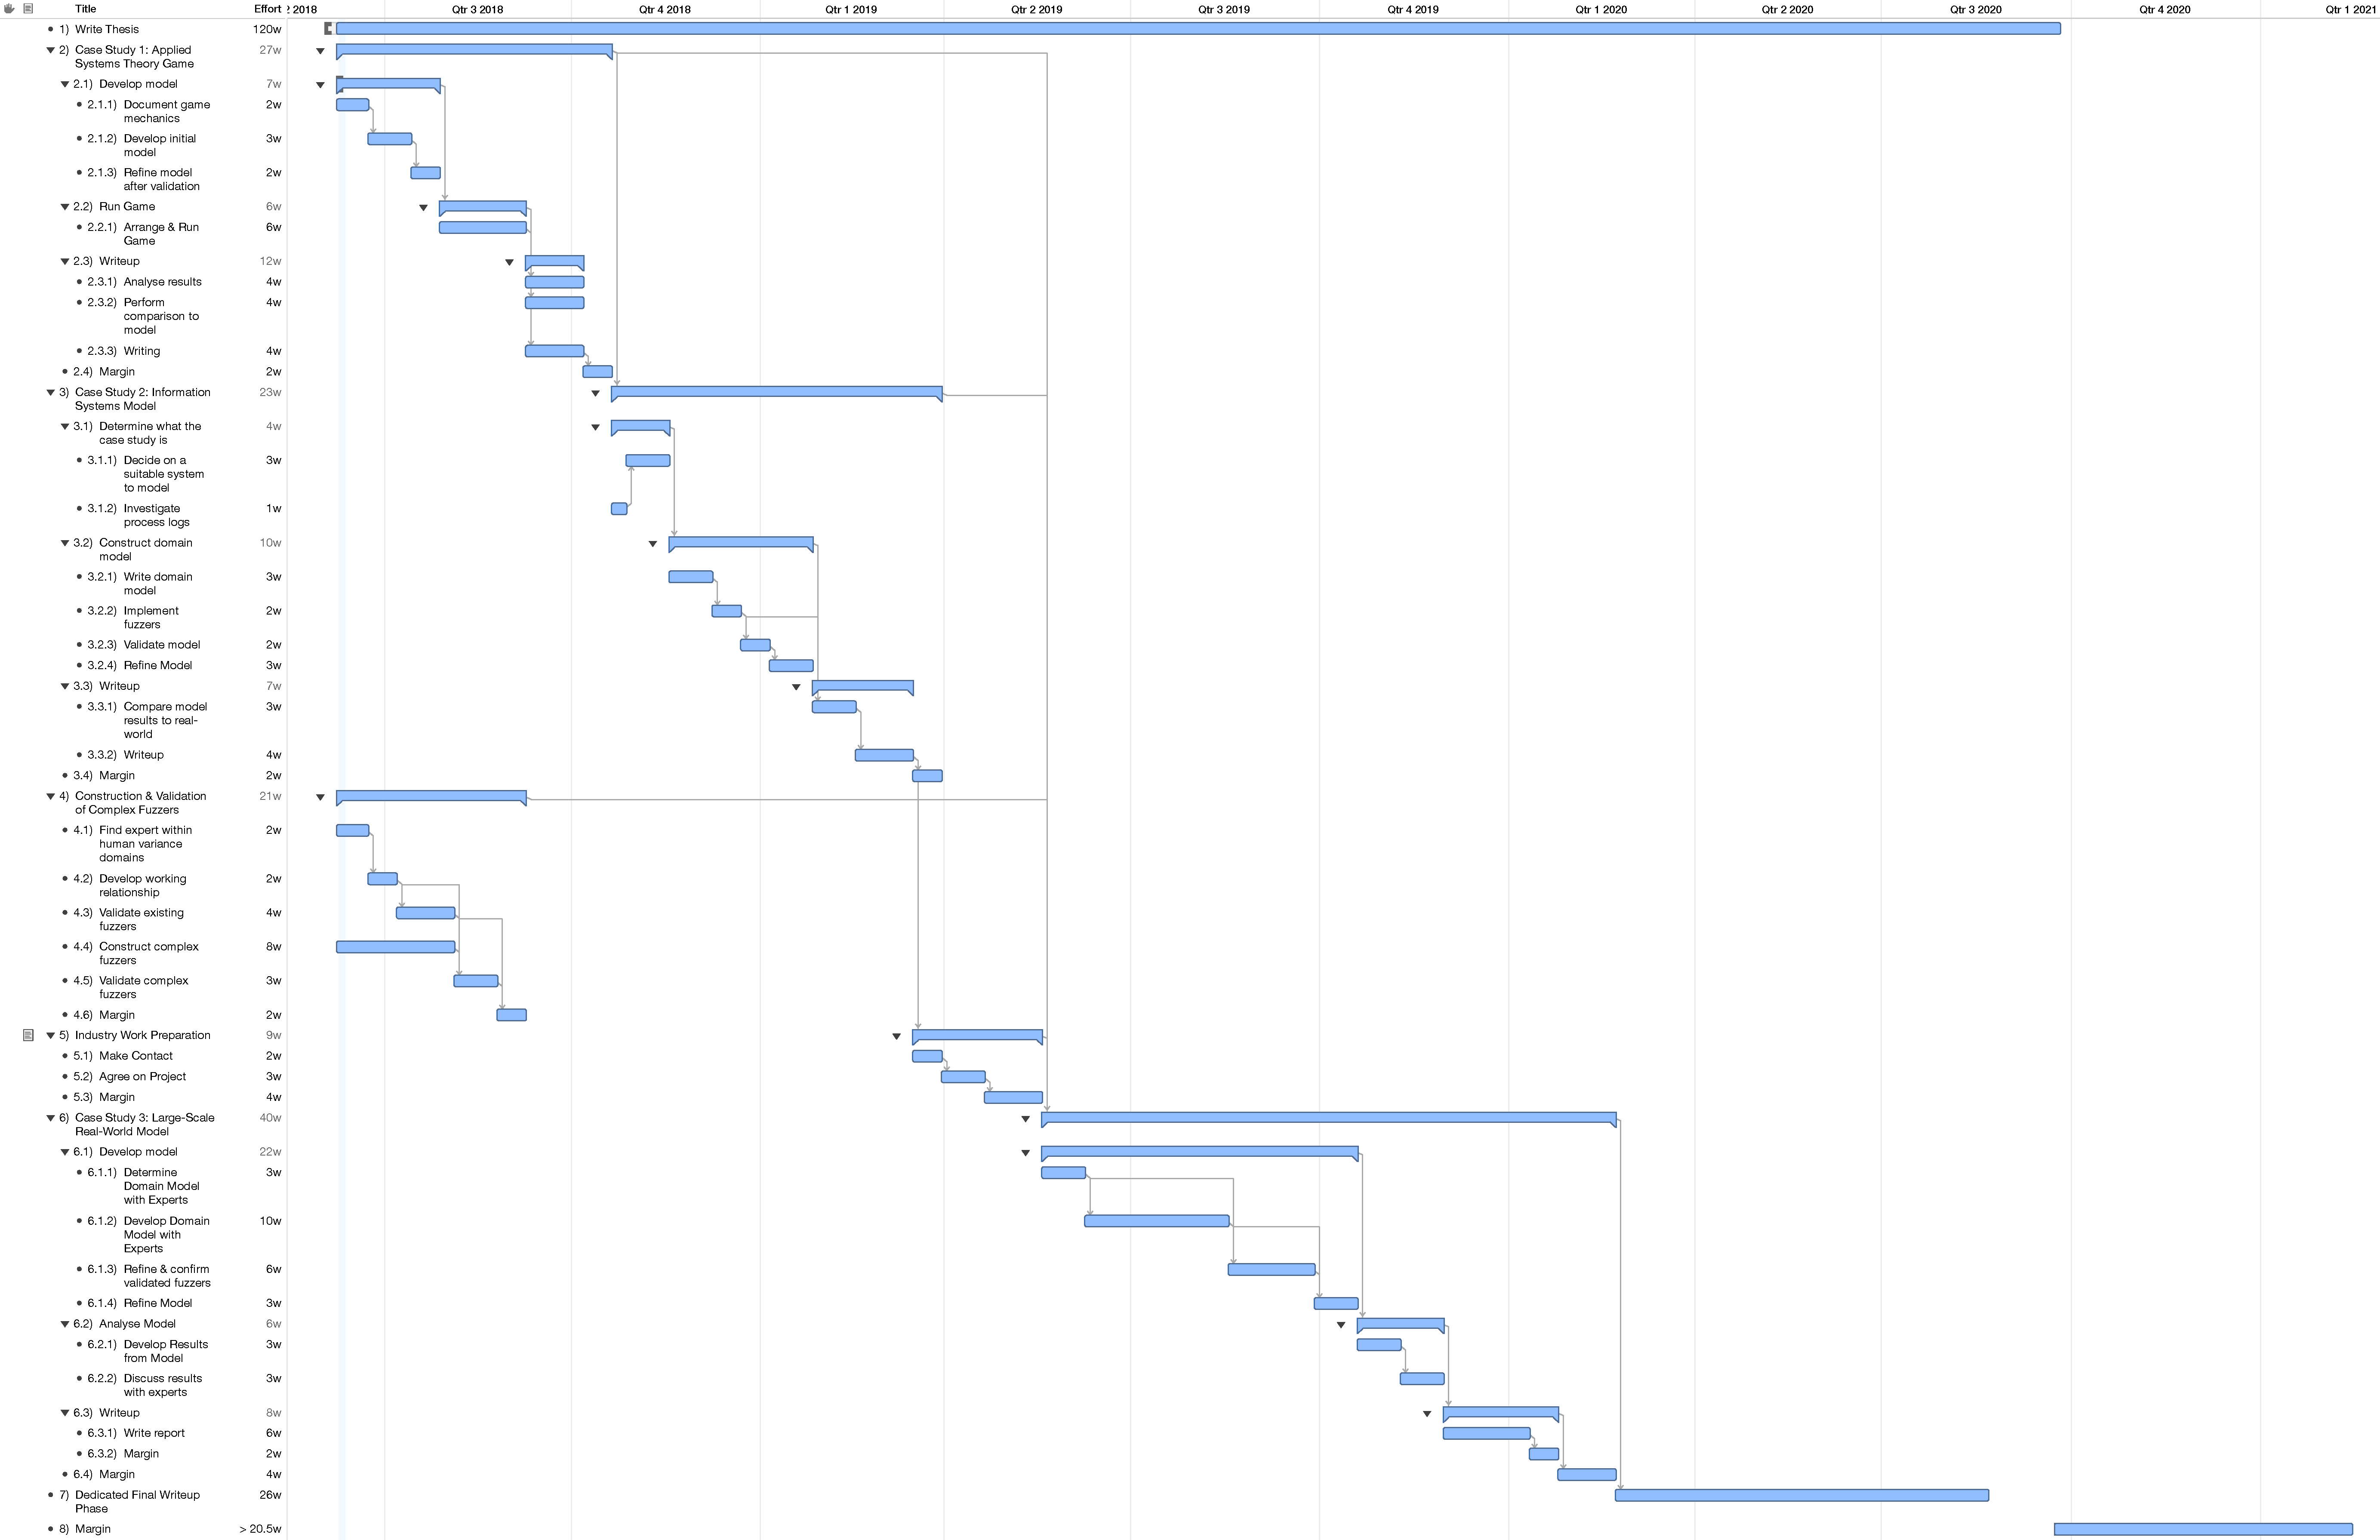
\includepdf[pagecommand=\section*{Appendix 4: Project Plan}]{gantt.pdf}


\end{document}